\section{Entropy}\label{sec:Entropy}
\subsection{Clausius Inequality}\label{subsec:Clausius_Inequality}
We have 2 equations for the efficiency of a \nameref{def:Carnot_Cycle}.
\begin{align*}
  \Efficiency_{\text{Carnot}} &= \frac{\Temp_{H} - \Temp_{L}}{\Temp_{H}} = 1 - \frac{\Temp_{L}}{\Temp_{H}} \\
                              &= \frac{\Heat_{H} - \Heat_{L}}{\Heat_{H}} = 1 - \frac{\Heat_{L}}{\Heat_{H}}
\end{align*}

\subsubsection{Reversible Carnot Cycles}\label{subsubsec:Reversible_Carnot_Cycles}
If we equate these (set them equal to each other) we get:
\begin{align*}
  1 - \frac{\Temp_{L}}{\Temp_{H}} &= 1 - \frac{\Heat_{L}}{\Heat_{H}} \\
  \frac{\Temp_{L}}{\Temp_{H}} &= \frac{\Heat_{L}}{\Heat_{H}} \\
  \frac{\Heat_{L}}{\Temp_{L}} &= \frac{\Heat_{H}}{\Temp_{H}} \\
  \frac{\Heat_{L}}{\Temp_{L}} - \frac{\Heat_{H}}{\Temp_{H}} &= 0
\end{align*}

This derivation's result is valid for any \nameref{def:Reversible_Process} which is a \nameref{def:Carnot_Cycle}.

\subsubsection{Irreversible Carnot Cycles}\label{subsubsec:Irreversible_Carnot_Cycles}
Looking at the energy balance present for an \nameref{def:Irreversible_Process}
\begin{equation*}
  \Heat_{H} - \Heat_{L} = \Work_{Out} + \Work_{\text{Friction}}
\end{equation*}

Because of the presence of $\Work_{\text{Friction}}$, $\Heat_{L}$ gets smaller (in comparison to a reversible Carnot cycle).
That means that the heat/temperature ratio equation has changed.
\begin{equation*}
  \frac{\Heat_{L}}{\Temp_{L}} - \frac{\Heat_{H}}{\Temp_{H}} < 0
\end{equation*}

Here, we start getting into the topic of \nameref{def:Entropy} a little bit more.

\begin{equation}\label{eq:Clausius_Inequality}
  \sum\limits_{i} \frac{d \Heat_{i}}{\Temp_{i}} \leq 0
\end{equation}

There are some things to say about \Cref{eq:Clausius_Inequality}.
\begin{itemize}[noitemsep]
\item Assume that you know the directions for the heats.
\item The $\frac{d \Heat_{i}}{\Temp_{i}}$ is called \nameref{def:Entropy}, or $\Entropy$.
\item If we divide the \nameref{def:Entropy} by the mass, we have the \nameref{def:Specific_Entropy}, $\frac{\frac{d \Heat_{i}}{\Temp_{i}}}{\Mass}$.
\end{itemize}

\subsubsection{Heat Engines and the Clausius Inequality}\label{subsubsec:Heat_Engine_Clausius_Inequality}
If we imagine a heat engine running through a set of cycles, as shown in \Cref{fig:Heat_Engine_Clausius_Inequality}, then we can say some things about it.

\begin{figure}[h!tbp]
  \centering
  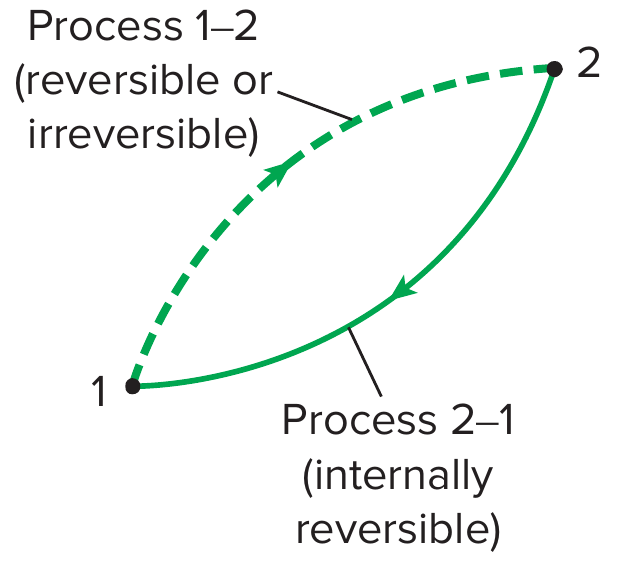
\includegraphics[scale=0.35]{Heat_Engine_Clausius_Inequality.png}
  \caption{Heat Engines and the Clausius Inequality (\cite[pg. 280]{ThermoTextbook})}
  \label{fig:Heat_Engine_Clausius_Inequality}
\end{figure}

Namely, the thing we can say is:
\begin{align*}
  \int\limits_{1}^{2} \frac{d \Heat}{\Temp} + \int\limits_{2}^{1} \frac{d \Heat}{\Temp} &\leq 0 \\
  \int\limits_{1}^{2} \Entropy + \int\limits_{2}^{1} \Entropy &\leq 0 \\
  (\Entropy_{1} - \Entropy_{2}) + \int\limits_{2}^{1} \Entropy &\leq 0 \\
  \Entropy_{2} - \Entropy_{1} &\geq \int\limits_{2}^{1} \frac{d \Heat}{\Temp}
\end{align*}

This last point is actually quite important and is restated here.
\begin{equation}\label{eq:Reversible_Process_Entropy_Lost}
  \Entropy_{2} - \Entropy_{1} \geq \int\limits_{2}^{1} \frac{d \Heat}{\Temp}
\end{equation}

\Cref{eq:Reversible_Process_Entropy_Lost} states that for an \nameref{def:Irreversible_Process}, \nameref{def:Work} is lost \textbf{forever}.
\begin{itemize}[noitemsep]
\item For \nameref{def:Irreversible_Process}es, $\Entropy$ \textbf{always} increases.
\item For \nameref{def:Reversible_Process}es, $\Change{\Entropy} = 0$.
\end{itemize}

%%% Local Variables:
%%% mode: latex
%%% TeX-master: "../../MMAE_320-Thermo-Reference_Sheet"
%%% End:


\subsubsection{Entropy and its Definitions}\label{subsec:Entropy_Definitions}
\begin{definition}[Entropy]\label{def:Entropy}
  \emph{Entropy} is an thermodynamically \nameref{def:Extensive_Property}.
  It is defined from the \nameref{subsec:Clausius_Inequality}, in \Cref{eq:Clausius_Inequality}.
  \begin{equation}\label{eq:Entropy}
    \Entropy = \frac{\Heat_{i}}{\Temp_{i}}
  \end{equation}

  Another equation to describe entropy is based on the concept of the number of energy states.
  \begin{equation}\label{eq:Entropy_Energy_States}
    \Entropy = \BoltzmannConstant \ln(W)
  \end{equation}
  where:
  \begin{description}[noitemsep]
  \item $\BoltzmannConstant$ is Boltzmann's Constant.
  \item $W$ is the number of energy states in the system.
    This value is usually proportional to temperature or some energy.
  \end{description}
\end{definition}

\begin{definition}[Specific Entropy]\label{def:Specific_Entropy}
  \emph{Specific Entropy}, like all the other specific properties of a state, is a thermodynamically \nameref{def:Intensive_Property}.
  Similarly to \nameref{def:Entropy}, specific entropy is defined from the \nameref{subsec:Clausius_Inequality}, in \Cref{eq:Clausius_Inequality}, but is also divided by the mass.
  \begin{equation}\label{eq:Entropy}
    \SpecificEntropy = \frac{\frac{\Heat_{i}}{\Temp_{i}}}{\Mass}
  \end{equation}
\end{definition}

There also exist \nameref{def:Cycle}s where the \nameref{def:Entropy} remains constant (which only happens if the \nameref{def:Process} is a \nameref{def:Reversible_Process}), which are called \nameref{def:Isentropic}.
These can only occur if the \nameref{def:Process} is \nameref{def:Adiabatic}.

\begin{definition}[Isentropic]\label{def:Isentropic}
  An \emph{isentropic} \nameref{def:Process}/\nameref{def:Cycle} has constant \nameref{def:Entropy}.
\end{definition}

\begin{example}[Textbook Problem 8.38]{Isentropic Ideal Gases}
  $\Mass = \SI{1}{\lbm}$ R-134a is expanded \nameref{def:Isentropic}ly in a \nameref{def:Closed_System} that goes from $\Pressure_{1} = \SI{100}{\psia}$ and $\Temp_{1} = \SI{100}{\degreeF}$ to $\Pressure_{2} = \SI{10}{\psia}$.
  Determine the total heat transfer and the work required for this \nameref{def:Process}?
  \tcblower{}
  \textbf{Concepts:} \\
  This is a \nameref{def:Closed_System}, so mass is constant, there is \textbf{no} mass flow.
  However, there can still be a heat and work flow. \\
  We are told this is an \nameref{def:Isentropic} process, so there is no change in temperature.
  \begin{align*}
    \Temp_{1} &= \Temp_{2} \\
    \Change{\Entropy} &= 0 \\
    \frac{\Change{\Heat}}{\Temp} &= 0 \\
    \Change{\Heat} &= 0
  \end{align*}

  There is a change in pressure, meaning the vessel itself expands.

  \textbf{Explore:} \\
  Pressure is \textbf{not} constant. \\
  The vessel is expanding, meaning there needs to be a change in energy.
  The energy is coming from the internal energy, $\InternalEnergy$, of the gas because the R-134a is not ``pushing'' against anything. \\
  We discovered that $\Change{\Heat} = 0$. \\
  We are not told about any work in, so assume $\Work_{In} = 0$.

  The energy balance is now:
  \begin{equation*}
    -\Work_{Out} = \Mass (\SpecificInternalEnergy_{2} - \SpecificInternalEnergy_{1}) \\
  \end{equation*}

  We can use Tables A.11E through A.13E to find values for R-134a.

  \textbf{Plan:} \\
  Using the pressures and temperatures, use the Tables to find the entropies and the internal energies.
  Remember that $\SpecificEntropy_{1} = \SpecificEntropy_{2}$, so we can find the different internal energies.

  \textbf{Solve:} \\
  Start by using Table A.13E at $\Pressure_{1} = \SI{100}{\psia}$ and $\Temp_{1} = \SI{100}{\degreeF}$ to find the initial properties of the R-134a.
  \begin{align*}
    \SpecificEntropy_{1} &= \SI{0.22902}{\btu\per\lbm\per\rankine} \\
    \SpecificInternalEnergy_{1} &= \SI{109.46}{\btu\per\lbm}
  \end{align*}

  Now, using the facts that $\SpecificEntropy_{1} = \SpecificEntropy_{2}$, and $\Pressure_{2} = \SI{10}{\psia}$, we use Table A.13E again, looking for a $\SpecificEntropy_{2}$ that is as similar to $\SpecificEntropy_{1}$ as possible.
  \begin{align*}
    \SpecificEntropy_{2} &= \SI{0.22949}{\btu\per\lbm\per\rankine} \\
    \Temp_{2} &= \SI{-29.52}{\degreeF} \\
    \SpecificInternalEnergy_{2} &= \SI{113.02}{\btu\per\lbm}
  \end{align*}

  \textbf{Validate:} \\

  \textbf{Generalize:} \\

\end{example}

%%% Local Variables:
%%% mode: latex
%%% TeX-master: "../MMAE_320-Thermo-Reference_Sheet"
%%% End:
